\section{Мета роботи}
Набути навичок та практичного досвіду у розробці рекурсивних програм.

\section{Хід роботи}
1) Розробити рекурсивний та ітераційний алгоритми розв’язання індивідуального завдання. Визначити та порівняти час виконання відповідних функцій, зробити висновки:

\begin{figure}[h]
    \centering
    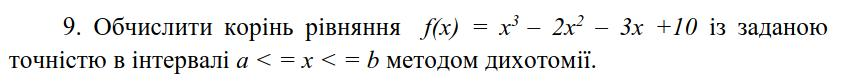
\includegraphics[width=16cm]{reports/algos/lab2/assets/1.png}
\end{figure}

2) Створюю базовий метод для обчислення значень моєї функції:

\begin{lstlisting}[style=customc]
#include <math.h>
#include <stdio.h>
#include <stdlib.h>
#include <time.h>

#include "general_utils.h"
    
double f(double x) { return x * x * x - 2 * x * x - 3 * x + 10; }
\end{lstlisting}

3) Створюю \textbf{ітераційний} алгоритм методу дихотомії:

\begin{lstlisting}[style=customc]
    double iterationBisection(double a, double b, double epsilon) {
        double mid = 0;
      
        if (f(a) * f(b) >= 0) {
          printf("The function has no root on that interval [%f, %f]\n", a, b);
          exit(0);
        }
      
        while ((b - a) >= epsilon) {
          mid = (a + b) / 2;
      
          if (fabs(f(mid)) <= epsilon) {
            break;
          }
      
          if (f(mid) * f(a) < 0) {
            b = mid;
          } else {
            a = mid;
          }
        }
      
        return mid;
    }
}
\end{lstlisting}


\clearpage
4) Створюю \textbf{рекурсивний} алгоритм методу дихотомії:

\begin{lstlisting}[style=customc]
    double recursiveBisection(double a, double b, double epsilon) {
        double mid = (a + b) / 2;
      
        if (fabs(f(mid)) <= epsilon) {
          return mid;
        }
      
        if (f(a) * f(b) >= 0) {
          printf("The function has no root on that interval [%f, %f]\n", a, b);
          exit(0);
        }
      
        if ((b - a) < epsilon) {
          return mid;
        } else if (f(mid) * f(a) < 0) {
          return recursiveBisection(a, mid, epsilon); 
        } else {
          return recursiveBisection(mid, b, epsilon); 
        }
    }
}
\end{lstlisting}

5) Створюю функцію яка буде тестувати \textbf{ітераційний} алгоритм:

\begin{lstlisting}[style=customc]
void iterationBisectionTest(double a, double b, double epsilon, int test_iterations) {
    double f_root = 0;
    double speed_time = 0, avg_speed_time = 0, avg_test = 0;
    clock_t start, end;

    for (size_t i = 0; i < test_iterations; i++) {
        start = clock();
        f_root = iterationBisection(a, b, epsilon);
        printf("The root of the equation on the interval \033[33m[%.2f, "
            "%.2f]\033[0m: %.2f\n",
            a, b, f_root);
        end = clock();
        speed_time = ((double)(end - start)) / CLOCKS_PER_SEC * 1000;
        printf("Function execution time: \033[32m%.3f\033[0m ms.\n\n", speed_time);
        avg_speed_time += speed_time;
    }

    avg_test = avg_speed_time / test_iterations;

    printf("AVERAGE EXECUTION TIME USING \033[34m%d\033[0m CALLS OF"
            "\033[34m ITERATIVE \033[0m"
            "METHOD IS: "
            "\033[32m%.3f\033[0m milliseconds.\n\n\n\n",
            test_iterations, avg_test);
}
\end{lstlisting}

\clearpage
6) Створюю функцію яка буде тестувати \textbf{рекурсивний} алгоритм:
    
\begin{lstlisting}[style=customc]
void recursiveBisectionTest(double a, double b, double epsilon, int test_iterations) {
    double f_root = 0;
    double speed_time = 0, avg_speed_time = 0, avg_test = 0;
    clock_t start, end;

    for (size_t i = 0; i < test_iterations; i++) {
        start = clock();
        f_root = recursiveBisection(a, b, epsilon);
        printf("The root of the equation on the interval \033[33m[%.2f, "
            "%.2f]\033[0m: %.2f\n",
            a, b, f_root);
        end = clock();
        speed_time = ((double)(end - start)) / CLOCKS_PER_SEC * 1000;
        printf("Function execution time: \033[32m%.3f\033[0m ms.\n\n", speed_time);
        avg_speed_time += speed_time;
    }

    avg_test = avg_speed_time / test_iterations;

    printf("AVERAGE EXECUTION TIME USING \033[34m%d\033[0m CALLS OF"
            "\033[34m ITERATIVE \033[0m"
            "METHOD IS: "
            "\033[32m%.3f\033[0m milliseconds.\n\n\n\n",
            test_iterations, avg_test);
}
\end{lstlisting}

7) Запускаю у головній функції виконання тестуючих методів, які в свою чергу, запустять обидва види алгоритму декілька разів та ми отримаємо:
\begin{itemize}
    \item по декілька запусків кожного з алгоритмів з однаковими параметрами.
    \item час виконання кожного запуску алгоритму.
    \item середній час виконання порції алгоритмів для більш детальних результатів.
\end{itemize} 

\begin{lstlisting}[style=customc]
void task1() {
  double a = -70, b = 70, epsilon = 0.0001, test_iterations = 5;

  highlightText("Iterative bisection algorythm:", "blue");
  iterationBisectionTest(a, b, epsilon, test_iterations);

  highlightText("Recursive bisection algorythm:", "blue");
  recursiveBisectionTest(a, b, epsilon, test_iterations);
}
\end{lstlisting}

\clearpage
\noindent 7) Результати з параметрами \(a = -5\), \(b = 5\), \(\epsilon = 0.0001\) на 5 повторів:
\begin{figure}[h]
    \centering
    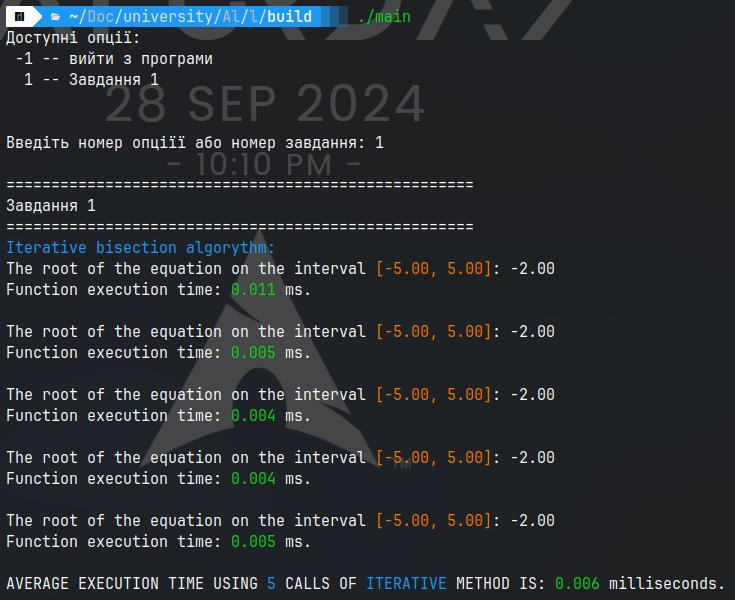
\includegraphics[width=14cm]{reports/algos/lab2/assets/2.png}
\end{figure}

\begin{figure}[h]
    \centering
    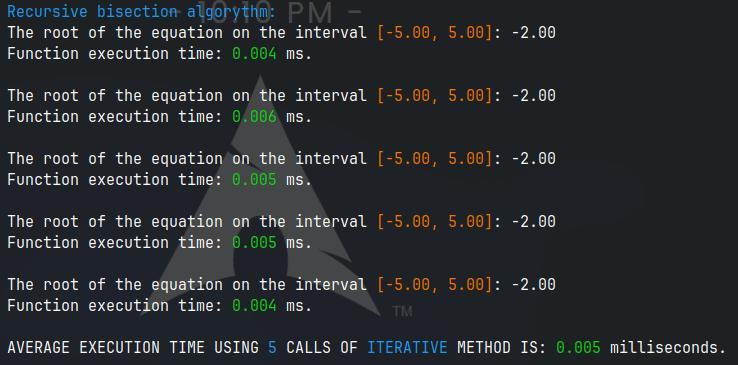
\includegraphics[width=14cm]{reports/algos/lab2/assets/3.png}
\end{figure}

\clearpage
\noindent 8) Результати з параметрами \(a = -20\), \(b = 20\), \(\epsilon = 0.0001\) на 5 повторів:
\begin{figure}[h]
    \centering
    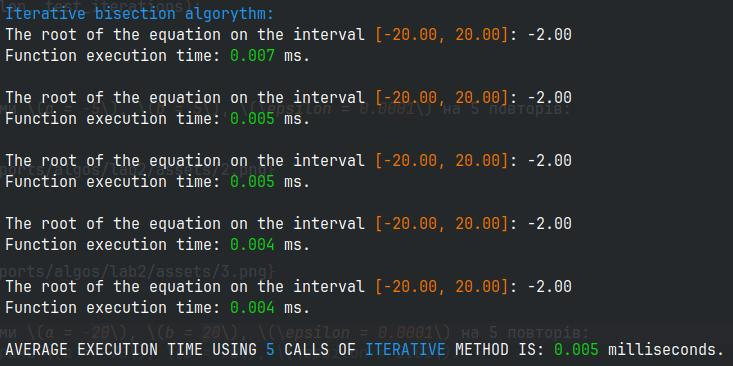
\includegraphics[width=14cm]{reports/algos/lab2/assets/4.png}
\end{figure}

\begin{figure}[h]
    \centering
    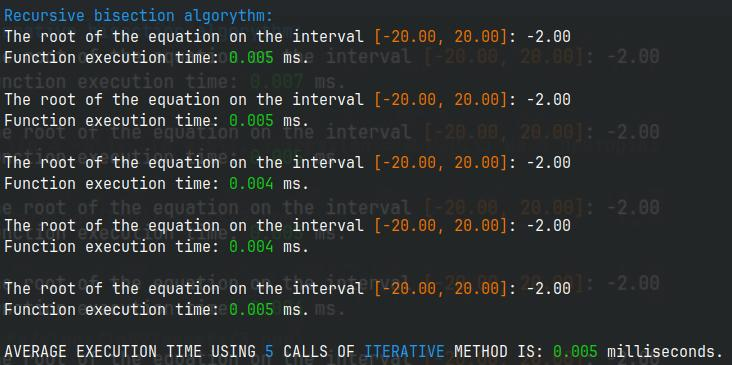
\includegraphics[width=14cm]{reports/algos/lab2/assets/5.png}
\end{figure}

\clearpage
\noindent 9) Результати з параметрами \(a = -70\), \(b = 70\), \(\epsilon = 0.0001\) на 10 повторів:
\begin{figure}[h]
    \centering
    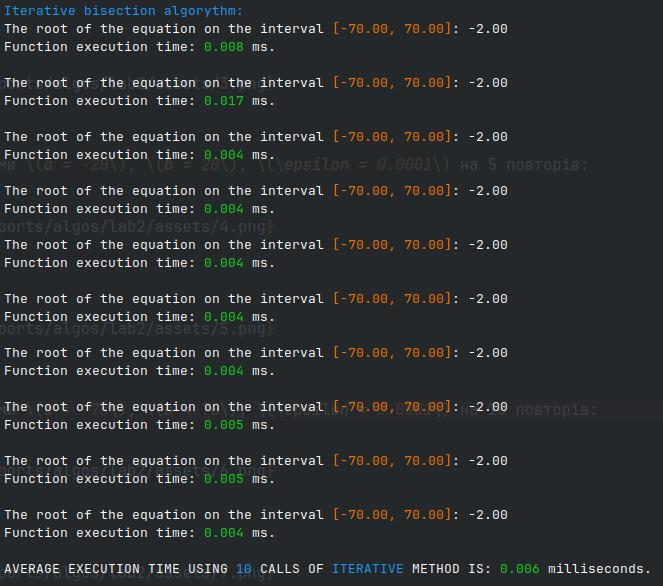
\includegraphics[width=10.5cm]{reports/algos/lab2/assets/6.png}
\end{figure}

\begin{figure}[h]
    \centering
    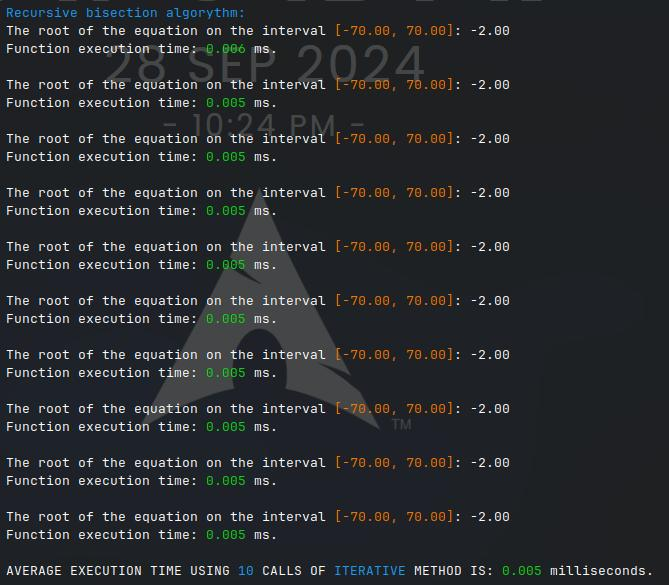
\includegraphics[width=10.5cm]{reports/algos/lab2/assets/7.png}
\end{figure}

\clearpage
\noindent 10) Також проведено декілька тестів з різною кількістю викликів алгоритмів:

\begin{figure}[h!]
    \centering
    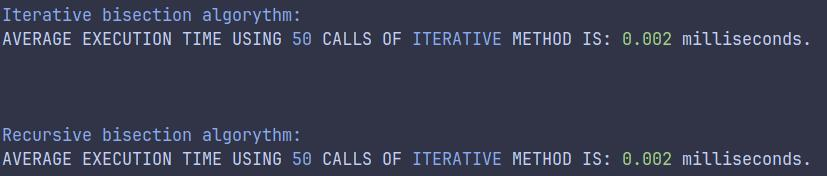
\includegraphics[width=13cm]{reports/algos/lab2/assets/8.png}
\end{figure}

\begin{figure}[h!]
    \centering
    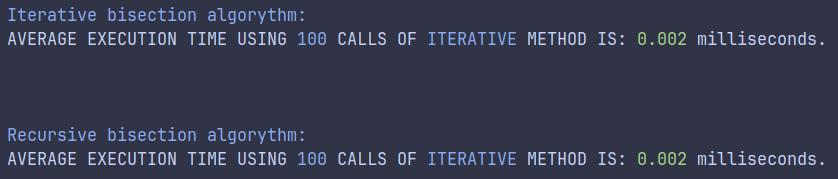
\includegraphics[width=13cm]{reports/algos/lab2/assets/9.png}
\end{figure}

\begin{figure}[h!]
    \centering
    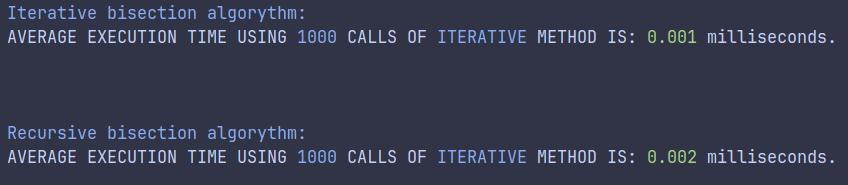
\includegraphics[width=13cm]{reports/algos/lab2/assets/10.png}
\end{figure}

\begin{figure}[h!]
    \centering
    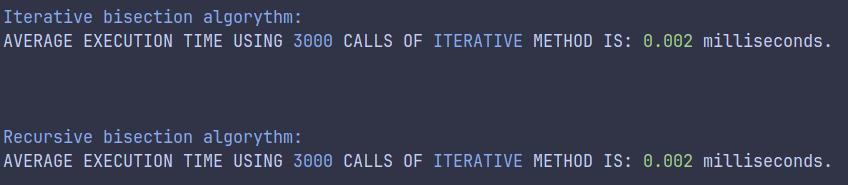
\includegraphics[width=13cm]{reports/algos/lab2/assets/11.png}
\end{figure}

\clearpage
\section{Висновки}
В ході виконання лабораторної роботи я реалізував метод дихотомії у рекурсивному та ітераційному виді. Можу зазначити що ітераційний та рекурсивний метод майже не мають сильної різниці коли відпрацьовують багато разів, результати виходять схожі. Але в окремих одиничних випадках все ж таки рекурсивний метод виявляється трішки швидкішим, але повільнішим при великому виклику рекурсивних процедур.